\chapter{Statistical modelling}

\textcite[p. 311]{fisher1922mathematical} stated that the objective of
statistics is to reduce the data since its volume is impossible 
to comprehend. In that sense, few quantities, generally parameters, 
should represent the whole phenomenon catching the most relevant information. 
Years later, Newman studied the theory of modelling which chan be divided 
in three aspects \cite[p. 161]{lehmann2012model}: 

\begin{enumerate}
  \item Models of complex phenomena are created by putting together 
  simple building elements that the researcher is familiar with and can 
  handle; 
  \item There are two types of models: the \textit{explanatory models}, 
  which will be focused on this work, and the \textit{interpolatory formulae}. 
  \item An explanatory theory necessitates a thorough understanding 
  of the problem's scientific context. In this regard, we investigated 
  this kind of problem involving Respondent-driven sampling and prevalence
  estimation as introduced in Chapter \ref{ch:theoretical-background}. 
\end{enumerate}

In this chapter, we develop models that enclose these ideas building each 
block separately. For a Bayesian modelling, we assume that each parameter
of the model has a probability distribution that incorporates the 
researcher's uncertainty about it. For each individual, we observe $k$ 
covariates that are possible risk factors represented by the vector 
$\x_i \in \R^{k}$ of the $i^{th}$ individual. We denote $\theta_i$ the 
probability of the $i$-th individual have been exposed to the disease
that depends on the prevalence $\theta$ and $\x_i$. \improve{We also 
consider when it depends on a spatial random effect caused by the 
connections analysed by the RDS.} The probability of positive test 
in the $i^{th}$ individual is denoted by $p_i$.  

Another important feature of the model is that sensitivity and 
specificity have the same distribution for all individuals and 
it only depends on the test used to diagnose. This is an assumption 
that must be analysed for the studied disease. For instance, COVID-19 
tests have different sensibilities and specificities for symptomatic and 
asymptomatic individuals.  

From above, we develop three different models: the first considers perfect 
tests, that is, $\gamma_s = \gamma_e = 1$ and no spatial random effect; 
the second considers imperfect tests, regarding $\gamma_s$ and $\gamma_e$, 
but ignoring the RDS structure; and the third one has imperfect tests and 
RDS structure. 

\section{Perfect tests}

The first model supposes the samples are independent and the test is perfect,
which means that $\theta_i = p_i$ for all $i$. Therefore it only considers the risk factors $\x_i$. 

\begin{equation}
  \begin{aligned}
    T_i &\sim \bern(\theta_i), \\
    g(\theta_i) &= g(\theta) + \x_i^T\beta, 
  \end{aligned}  
\end{equation}
where $v^T$ denotes the transpose of $v$, and $g(\cdot)$ is a link function.
The parameter $\beta \in \R^{k}$ is the risk effects. For Bayesian inference, priors on
$\beta$ and $\theta$ must be included. We use $\beta ~ \sim \N(\mu, \Sigma)$
and $\theta \sim \betadist(a^{p}, b^p)$, where $\mu
\in \R^{k}$, $\Sigma \in \R^{k\times k}$ symmetric positive-definite matrix,
$a^p \in \R_{++}$, and $b^p \in \R_{++}$
are fixed hyperparameters. 

\begin{remark}
  If the risk factors are zero, i.e $\x_i = 0$, the probability of the
  $i^{th}$ having been exposed is the prevalence $\theta$, which means that in
  a population with no risk effects, the probability of a person has the
  disease is exactly the proportion in this population. 
\end{remark}

\subsection{Identifiability}

\subsection{Toy example}

\section{Sensitivity and specificity}

In this section, we describe a model to infer about sensitivity 
and specificity separately from the final model for prevalence 
estimation. This is interesting 
to experiment and analyse different prior specification approaches. 
The model is the following: suppose having a gold standard 
test for a disease and we want to estimate the sensitivity and 
specificity of another simpler and faster test. In a population, 
with the gold standard, it's impossible to differentiate the true 
negatives from the true positives - in this scenario, ``true'' means 
the decision of the gold standard. However not all diseases have a 
perfect gold standard. Therefore, we denote 
\begin{gather*}
  y_{negative} \sim \operatorname{Binomial}(n_{\gamma_e}, \gamma_e), \\
  y_{positive} \sim \operatorname{Binomial}(n_{\gamma_s}, \gamma_s),
\end{gather*}
such that $y_{negative}$ are negative tests on known negative 
subjects and $y_{positive}$ are positive tests on
known positive. In a classic Bayesian analysis, we have to define a 
prior distribution for the parameters $(\gamma_e, \gamma_s) \sim \pi(\gamma_e,
\gamma_s)$. 

For this, we consider three different approaches: 

\begin{enumerate}
  \item Treating each parameter as independent with a beta distribution 
  with pre-specified hyperparameters. 
  \item Hierarchical partial pooling, when dealing with more studies. 
  \item A Bivariate Beta (see Appendix
  \ref{appendix:bivariate-beta-distribution}) 
  distribution.
\end{enumerate}

When considering separated experiments for specificity and
sensitivity, there is
no information about their correlation, which is the case for our model. Then we define the the prior distributions
\begin{gather*}
  \gamma_e \sim \operatorname{Beta}(a_e, b_e), \\
  \gamma_s \sim \operatorname{Beta}(a_s, b_s), \\
  \theta \sim \operatorname{Beta}(a_{\theta}, b_{\theta}).
\end{gather*} 
Using data from \cite{bennett2020estimating} about COVID-19 seroprevalence in
Santa Clara:  
\begin{align*}
  y/n &= 50/3330,\\
y_{negative}/n_{\gamma_e} &= 399/401, \\
y_{positive}/n_{\gamma_s} &= 103/122, 
\end{align*}
we fit the model and obtain the results showed in Figure
\ref{fig:results-posterior-model1}. All the codes were done in {\em Stan} and
{\em PyStan}.

\begin{figure}[!ht]
  \centering
  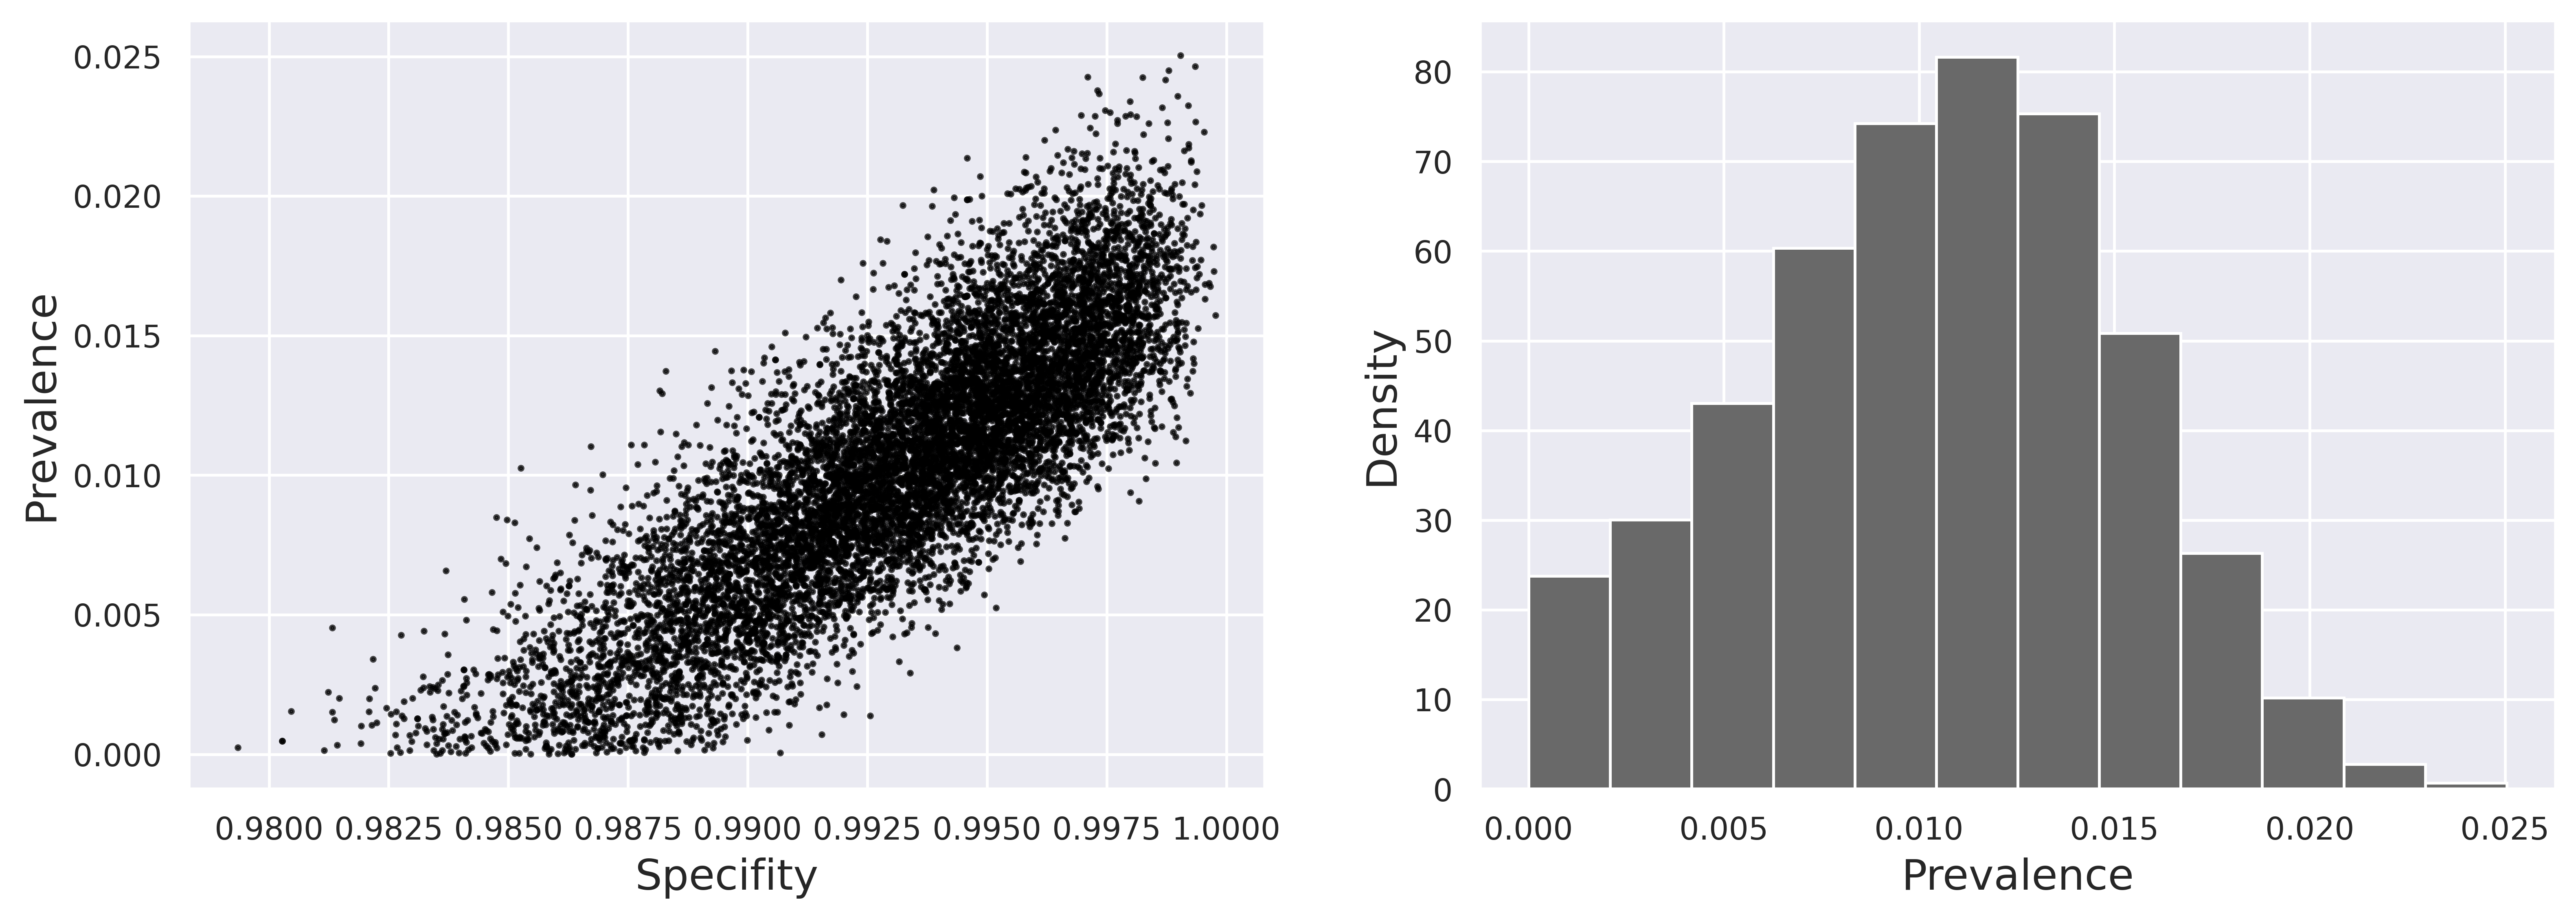
\includegraphics[width=\textwidth]{../../images/model1_gelman_figure_english.png}
  \caption{Scatter plot of posterior simulations of prevalence against
  specificity and histogram of posterior simulations of the prevalence.}
  \label{fig:results-posterior-model1}
\end{figure}

Other approach considers more than one study about specificity and
sensitivity. A {\em hierarchical partial pooling} model for these studies
can be done in the following way: 
\begin{gather*}
    \operatorname{logit}(\gamma_s^j) \sim \operatorname{Normal}(\mu_{\gamma_s}, \sigma_{\gamma_s}), \\
    \operatorname{logit}(\gamma_e^j) \sim \operatorname{Normal}(\mu_{\gamma_e}, \sigma_{\gamma_e}), 
\end{gather*}
for $1 \le j \le K$ studies, such that the first study is the considered one.
Partial pooling because the parameters can be sampled from the same
distribution. Hierarchical because the parameters of this distribution have
its one prior distributions. For instance, 
\begin{align*}
    \mu_{\gamma_s} &\sim N(0, 10), \\ 
    \mu_{\gamma_e} &\sim N(0, 10), \\
    \sigma_{\gamma_s} &\sim N^+(0,1), \text{ and } \\
    \sigma_{\gamma_e} &\sim N^+(0,1),
\end{align*}
where $N^+(a,b)$ is the truncated normal distribution in $[0,+\infty)$. All
the codes available at Github
repository\footnote{\url{https://github.com/lucasmoschen/rds-bayesian-analysis}}.

Finally, we studied a joint distribution for specificity and sensitivity, a
possible bivariate beta distribution built in \cite{olkin2015constructions}.
This distribution is derived from a Dirichlet distribution of order four. Let $U = (U[1],...,U[4]) \sim \operatorname{Dirichlet}(\boldsymbol{\alpha})$, where
$\boldsymbol{\alpha} \in \mathbb{R}^4_+$. Therefore, defining $X = U[1] +
U[2]$ and $Y = U[1] + U[3]$, we will have that $(X,Y)$ has a well-defined
probability distribution in
$[0,1] \times [0,1]$ such that $X$ and $Y$ have marginally beta distributions,
and they have correlation in all space. Depending on the definition of
$\boldsymbol{\alpha}$, the correlation between the variables range from -1 and
1. Figure \ref{fig:beta-bivariate} shows some examples of this construction. 

\begin{figure}[!ht]
    \centering
    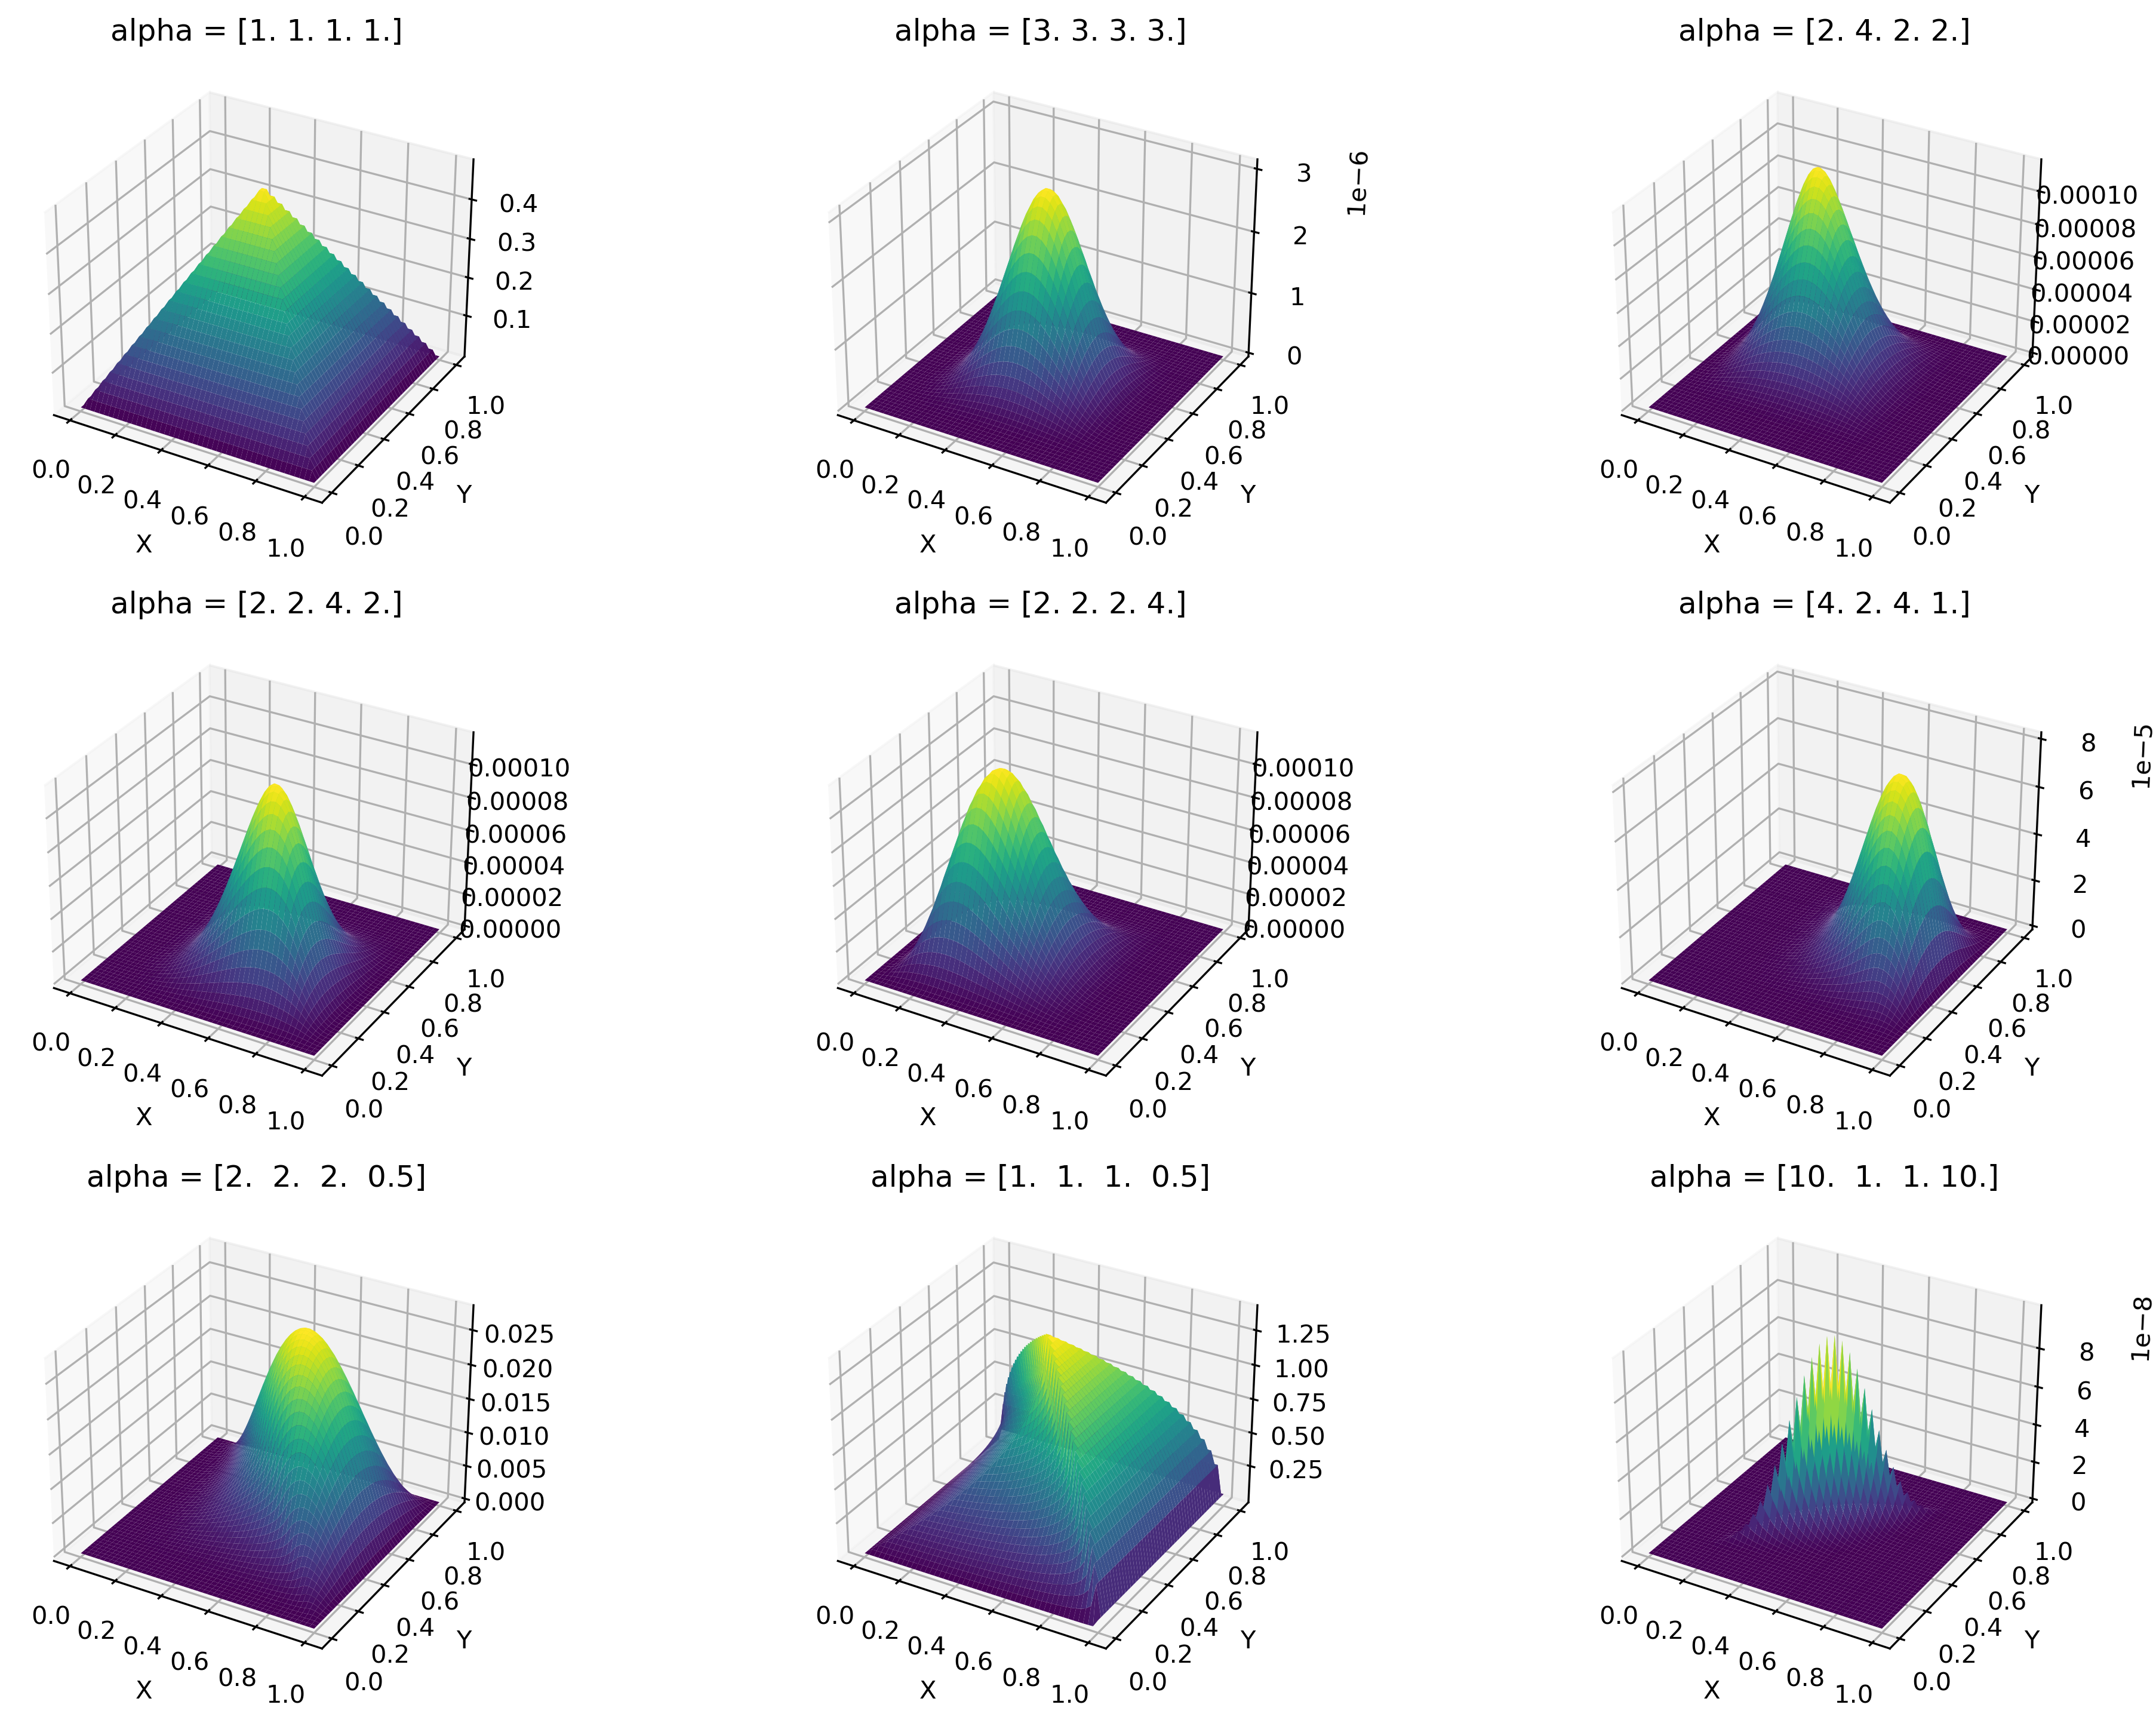
\includegraphics[width=\textwidth]{beta-distributions.png}
    \caption{Different choices of $\alpha$ and the joint distribution of the variables $X$ and $Y$.}
    \label{fig:beta-bivariate}
\end{figure}

In this section, we shall describe how to use the Bivariate Beta (see Appendix
\ref{appendix:bivariate-beta-distribution}) to model the correlation between
specificity and sensitivity.

\subsection{Specifying parameters
\texorpdfstring{$\boldsymbol{\alpha}$}{alpha}}

Suppose that the researcher has knowledge about the main moments of $X$ and
$Y$, such that $\ev(X) = m_1 \in (0,1), \ev(Y) = m_2 \in (0,1), \var(X) = v_1
\in (0, 1),$ and $\var(Y) =
v_2 \in (0,1)$. Notice that $v_1 + m_1^2 = \var(X_1) + \ev[X_1]^2 = \ev[X_1^2]$ and
$$
\ev[X_1^2] - \ev[X_1] = \frac{(\alpha_1 + \alpha_2 + 1)(\alpha_1 + \alpha_2)}{(\tilde{\alpha} + 1)\tilde{\alpha}} - \frac{\alpha_1 + \alpha_2}{\tilde{\alpha}} = -\frac{(\alpha_1 + \alpha_2)(\alpha_3 + \alpha_4)}{\tilde{\alpha}(\tilde{\alpha}+1)} < 0, 
$$
that is, $v_1 + m_1^2 - m_1 < 0 \implies v_1 < m_1 - m_1^2$ and similarly,
$v_2 < m_2 - m_2^2$. After fixing these quantities, we will have a non-linear system with four equations and four
unknown variables. Hence, we want to solve the following 
\begin{equation}
  \label{eq:system-moments-alpha}
  \begin{cases}
    m_1 = \dfrac{\alpha_1+\alpha_2}{\tilde{\alpha}} \\
    m_2 = \dfrac{\alpha_1+\alpha_3}{\tilde{\alpha}} \\ 
    v_1 = \dfrac{(\alpha_1+\alpha_2)(\alpha_3+\alpha_4)}{\tilde{\alpha}^2(\tilde{\alpha}+1)} = m_1\dfrac{\alpha_3+\alpha_4}{\tilde{\alpha}(\tilde{\alpha}+1)} \\
    v_2 = \dfrac{(\alpha_1+\alpha_3)(\alpha_2+\alpha_4)}{\tilde{\alpha}^2(\tilde{\alpha}+1)} = m_2\dfrac{\alpha_2+\alpha_4}{\tilde{\alpha}(\tilde{\alpha}+1)}.
  \end{cases}
\end{equation}

\begin{proposition}
  System \eqref{eq:system-moments-alpha} has a solution if, and only if, the relation
  \begin{equation}
    \label{eq:v2}
    v_2 = \frac{(1 - m_2)\tilde{\alpha}}{\tilde{\alpha}(\tilde{\alpha}+ 1)} = \frac{1 - m_2}{\frac{m_1 - m_1^2}{v_1}} = \frac{v_1(1 - m_2)}{m_1(1-m_1)},
  \end{equation}
  is satisfied. When there is a solution, there will be
  infinitely many and they all lay in the ray 
  $$
\mathcal{L} = \{(1,-1,-1,1)\alpha_4 + k : \alpha_4 > 0\}, 
$$
such that $k = \left((m_1 + m_2 - 1)\tilde{\alpha}, (1-m_2)\tilde{\alpha},
(1-m_1)\tilde{\alpha}, 0\right)$. 
\end{proposition}

\begin{proof}

The first two equations of the system \eqref{eq:system-moments-alpha} can be
rewritten as a linear system:
\begin{align*}
  (m_1 - 1)\alpha_1 + (m_1 - 1)\alpha_2 + m_1\alpha_3 + m_1\alpha_4 &= 0 \\
  (m_2 - 1)\alpha_1 + m_2\alpha_2 + (m_2-1)\alpha_3 + m_2\alpha_4 &= 0,   
\end{align*}
which is equivalent to 
\begin{align*}
  \alpha_1 + \alpha_2 + \frac{m_1}{m_1-1}\alpha_3 + \frac{m_1}{m_1-1}\alpha_4 &= 0 \\
  \alpha_2 + \frac{1-m_2}{m_1-1}\alpha_3 + \frac{m_1-m_2}{m_1-1}\alpha_4 &= 0.
\end{align*}
Then, we can write $\alpha_1$ and $\alpha_2$ as functions of $\alpha_3$ and
$\alpha_4$:
\begin{align}
  \alpha_1 &= \frac{m_1+m_2-1}{1-m_1}\alpha_3 + \frac{m_2}{1-m_1}\alpha_4 \\
  \alpha_2 &= \frac{1-m_2}{1-m_1}\alpha_3 + \frac{m_1-m_2}{1-m_1}\alpha_4.
\end{align}
With that expression, let $\alpha_1 = a_3\alpha_3 + a_4\alpha_4$ and $\alpha_2
= b_3\alpha_3 + b_4\alpha_4$. Denote $c_3 = a_3 + b_3 + 1$ and $c_4 = a_4 +
b_4 + 1$. Then, consider the third equation of the system
\eqref{eq:system-moments-alpha}, 
\begin{equation*}
  \begin{split}
    &\frac{v_1}{m_1} = \frac{\alpha_3+\alpha_4}{\tilde{\alpha}(\tilde{\alpha} +1)} = \frac{\alpha_3+\alpha_4}{(\alpha_1+\alpha_2+\alpha_3+\alpha_4)^2 + (\alpha_1+\alpha_2+\alpha_3+\alpha_4)} \\
     &\implies \frac{v_1}{m_1}(\alpha_1 + \alpha_2 + \alpha_3 + \alpha_4)^2 = \alpha_3 + \alpha_4 - \frac{v_1}{m_1}(\alpha_1 + \alpha_2 + \alpha_3 + \alpha_4) \\
    &\implies \frac{v_1}{m_1}(c_3\alpha_3 + c_4\alpha_4)^2 = \left(1-\frac{v_1}{m_1}c_3\right)\alpha_3 + \left(1-\frac{v_1}{m_1}c_4\right)\alpha_4 \\
    &\implies \frac{v_1c_3^2}{m_1}\alpha_3^2 + \left(\frac{2v_1c_3c_4\alpha_4+v_1c_3}{m_1} - 1\right)\alpha_3 + \left(\frac{v_1c_4^2\alpha_4^2 + v_1c_4\alpha_4}{m_1} - \alpha_4\right) = 0 \\ 
    &\implies v_1c_3^2\alpha_3^2 + (2v_1c_3c_4\alpha_4+v_1c_3 - m_1)\alpha_3 + (v_1c_4^2\alpha_4^2 + v_1c_4\alpha_4 - m_1\alpha_4) = 0.
  \end{split}
\end{equation*}
Using a Computer Algebra System (CAS) with the Python library SymPy, the above
expression can be simplified as follows:
$$
v_1\alpha_3^2 + \left(v_1(1-m_1) + 2v_1\alpha_4 - m_1(1-m_1)^2\right)\alpha_3 - \alpha_4m_1(1-m_1)^2 + \alpha_4v_1(1 - m_1) + v_1\alpha_4^2 = 0.
$$
This way, the solutions of the above equation are function of $\alpha_4$.
Therefore, after solving the equations, we can use the last equation of the
system \eqref{eq:system-moments-alpha} as a function on of $\alpha_4$. Let, 
$$
\Lambda = \left(v_1(1-m_1) + v_1\alpha_4 - m_1(1-m_1)^2\right).
$$
Then, 
\begin{equation*}
  \begin{split}
    \Delta &= \left(v_1(1-m_1) + 2v_1\alpha_4 - m_1(1-m_1)^2\right)^2 - 4v_1(\alpha_4v_1(1 - m_1) - \alpha_4m_1(1-m_1)^2 + v_1\alpha_4^2), \\
    &= \left(\Lambda + v_1\alpha_4\right)^2 - 4v_1\alpha_4\Lambda \\
    &= \Lambda^2 - 2\Lambda v_1\alpha_4 + (v_1\alpha_4)^2 \\
    &= (\Lambda - v_1\alpha_4)^2 \\
    &= \left(v_1(1-m_1) - m_1(1-m_1)^2\right)^2 \\ 
    &= (1 - m_1)^2(v_1 + m_1^2 - m_1)^2.
  \end{split}
\end{equation*}
Note that $v_1 + m_1^2 = \var(X_1) + \ev[X_1]^2 = \ev[X_1^2]$ and
$$
\ev[X_1^2] - \ev[X_1] = \frac{(\alpha_1 + \alpha_2 + 1)(\alpha_1 + \alpha_2)}{(\tilde{\alpha} + 1)\tilde{\alpha}} - \frac{\alpha_1 + \alpha_2}{\tilde{\alpha}} = -\frac{(\alpha_1 + \alpha_2)(\alpha_3 + \alpha_4)}{\tilde{\alpha}(\tilde{\alpha}+1)} < 0.
$$
Therefore, 
$$
\sqrt{\Delta} = (1-m_1)(m_1 - v_1 - m_1^2)
$$
and 
\begin{equation*}
  \begin{split}
    \alpha_3 &= \frac{1}{2v_1}\left(\left(m_1(1-m_1)^2 - v_1(1-m_1) - 2v_1\alpha_4\right) \pm (1-m_1)(m_1 - v_1 - m_1^2)\right) \\
    &= - \alpha_4 + \frac{(1-m_1)(m_1 - m_1^2 - v_1) \pm (1-m_1)(m_1-v_1-m_1^2)}{2v_1}.
  \end{split}
\end{equation*}
When the sign is negative, we have that $\alpha_3 = - \alpha_4$, an impossible
solution. Then, 
$$
\alpha_3 = \frac{(1-m_1)(m_1 - m_1^2 - v_1)}{v_1} - \alpha_4.
$$

We summarize the expressions in function of $\alpha_4$: 
\begin{align*}
  \alpha_3 &= \frac{(1-m_1)(m_1 - m_1^2 - v_1)}{v_1} - \alpha_4 \\
  \alpha_1 &= \frac{m_1+m_2-1}{1-m_1}\alpha_3 + \frac{m_2}{1-m_1}\alpha_4 = \frac{(m_1 + m_2 - 1)(m_1 - m_1^2 - v_1)}{v_1} + \alpha_4 \\
  \alpha_2 &= \frac{1-m_2}{1-m_1}\alpha_3 + \frac{m_1-m_2}{1-m_1}\alpha_4 = \frac{(1 - m_2)(m_1 - m_1^2 - v_1)}{v_1} - \alpha_4 .
\end{align*}

From here, one can calculate that
$$
\tilde{\alpha} = \frac{m_1 - m_1^2 - v_1}{v_1}.
$$
Since $\alpha_2 + \alpha_4 = (1 - m_2)\tilde{\alpha}$, we have that the last
equation of the system \eqref{eq:system-moments-alpha} is given by
\eqref{eq:v2}, that is, the system $\eqref{eq:system-moments-alpha}$ has a solution if and
only if, equation \eqref{eq:v2} is satisfied. If it is, the solution is the ray 
$$
\mathcal{L} = \{(1,-1,-1,1)\alpha_4 + k : \alpha_4 > 0\}, 
$$
such that $k = \left((m_1 + m_2 - 1)\tilde{\alpha}, (1-m_2)\tilde{\alpha},
(1-m_1)\tilde{\alpha}, 0\right)$. 

\end{proof}


Now change the fourth equation of \eqref{eq:system-moments-alpha} by: 
$$
\cor(X,Y) = \frac{\alpha_1\alpha_4 - \alpha_2\alpha_3}{\sqrt{(\alpha_1+\alpha_2)(\alpha_3+\alpha_4)(\alpha_1+\alpha_3)(\alpha_2+\alpha_4)}} = \frac{\alpha_1\alpha_4 - \alpha_2\alpha_3}{\tilde{\alpha}^2\sqrt{m_1m_2(1-m_1)(1-m_2)}}
$$

Supposing the expression for $\alpha_1, \alpha_2$ and $\alpha_3$, that is,
$m_1, m_2$ and $v_1$ are fixed, and supposing we fix $\rho = \cor(X,Y)$, we
can simplify the above expression (using a software) as follows: 

$$
\rho = \frac{1}{\tilde{\alpha}\sqrt{m_1m_2(1-m_1)(1-m_2)}}\alpha_4 - \sqrt{\frac{(1 - m_1)(1 - m_2)}{m_1m_2}},
$$
which is linear on $\alpha_4$, that is, for fixed values of
$m_1, m_2, v_1$ and $\rho$, there is an unique $\alpha_4$, and hence,
$\alpha_1, \alpha_2$ and $\alpha_3$ that satisfies system
\eqref{eq:system-moments-alpha} with the fourth equation changed by the
correlation. 

\section{Imperfect tests}

This model includes the sensitivity and specificity of the diagnostic test. 

\begin{equation}
  \begin{aligned}
    T_i &\sim \bern(p_i) \\
    p_i &= \gamma_s\theta_i + (1-\gamma_e)(1 - \theta_i),  \\
    g(\theta_i) &= g(\theta) + \x_i^T\beta,  \\
    \beta &\sim \N(\mu, \Sigma), \\ 
    \theta &\sim \betadist(a^p, b^p) \\
    \gamma_s &\sim \betadist(a^s, b^s), \\
    \gamma_e &\sim \betadist(a^e, b^e), \\    
  \end{aligned}  
\end{equation}
where $a^p, a^s, a^e, b^p, b^s, b^e \in \R_{++}$ are fixed hyperparameters.
This model does not include prior knowledge about the correlation between
specificity and sensitivity. 

\subsection{Toy example}

Consider the following model \cite{gelman2020bayesian}:
\begin{gather*}
  y \sim \operatorname{Binomial}(n, p), \\
  p = \theta\gamma_s + (1- \theta)(1-\gamma_e), 
\end{gather*}
such that $y$ is the number of positive tests in a population of size $n$. In
a Bayesian paradigm, a prior $\pi(\theta, \gamma_e, \gamma_s)$ must be
specified. For instance, $\pi(\theta, \gamma_e, \gamma_s) =
\pi(\theta)\pi(\gamma_e, \gamma_s)$ and $\theta \sim
\operatorname{Beta}(\alpha_{\theta}, \beta_{\theta})$, in which
$\alpha_{\theta}$ and $\beta_{\theta}$ are positive hyperparameters. Since the
three parameters $\theta, \gamma_e$, and $\gamma_s$ are not jointly
identifiable only from $y$, prior information on $\gamma_e$ and $\gamma_s$
need be added. 

\section{Imperfect tests and respondent-driven sampling}

For now, we consider the network dependence induced by the RDS with no
associated model. Therefore, we treat it as a random effect for
each individual. Conditionally autoregressive (CAR) models in the
Gaussian case are used. Let $[\tilde{Q}]_{ij} = \tilde{q}_{ij}$ be a fixed matrix which measures the distance between $i$
and $j$, and $\tilde{q}_{i+} = \sum_{j} \tilde{q}_{ij}$. In general, we use
$$
\tilde{q}_{ij} = \begin{cases}
  1, &\text{if } i \text{ recruited } j \text{ or the contrary} \\
  0, &\text{otherwise.} 
\end{cases}
$$
Next we define the scaled adjacency matrix $Q = D^{-1}\tilde{Q}$, such that $D$
is a diagonal matrix with $D_{ii} = \tilde{q}_{i+}$. Finally let $|\rho| < 1$ be a
parameter to controls the dependence between neighbors. Hence, we specify the
model as follows:

\begin{equation}
  \begin{aligned}
    T_i &\sim \bern(p_i) \\
    p_i &= \gamma_s\theta_i + (1-\gamma_e)(1 - \theta_i),  \\
    g(\theta_i) &= g(\theta) + \x_i^T\beta + \omega_i,  \\
    \omega_i|\{\omega_j\}_{j\neq i}, \tau &\sim \N\left(\rho\sum_j q_{ij}\omega_j, \tau^{-1}/\tilde{q}_{i+}\right) \\
    \beta &\sim \N(\mu, \Sigma), \\ 
    \theta &\sim \betadist(a^p, b^p) \\
    \gamma_s &\sim \betadist(a^s, b^s), \\
    \gamma_e &\sim \betadist(a^e, b^e), \\  
    \tau &\sim \operatorname{Gamma}(a^{\tau}, b^{\tau}).
  \end{aligned}  
\end{equation}
By Brook's Lemma \cite[]{brook1964distinction}, the joint distribution of
$\omega$ can be specified as 
$$
\omega \sim \N\left(0, \left[\tau (D - \rho \tilde{Q})\right]^{-1}\right).
$$

\subsection{Toy example}

\begin{enumerate}
  \item Between the model with the log odds of prevalence having a Gaussian prior
  distribution and the other with the prevalence having a Beta prior
  distribution, 
  the latter was usually faster and without divergences. Therefore the 
  preferable model is with the prevalence. 

  \item Non-centered distributions are really worst. 
  \item Comparison between parametrization of sigma and tau showed that
  they are similar in sight of time of execution, energy and divergences,
  among others diagnostics. However, the mean estimate of sigma is more
  controlled. The median estimate is very similar. This happens because there
  are a few very high samples for $\tau$ that will have high weight in the
  final result. Small samples for $\sigma$ have less impact, despite having
  some. 
  \item I observed that the RDS structure worsens the funil aspect of the
  scatter plot. Although the sparsity may cause divergence problems, which
  makes sense, sparsity and tree structure appears to be a bad feature for the
  model. Apparently there is no connection with the number of connected
  components. Test with one and five had similar results (actually they were
  better in the five case, but the difference can be random noise).
\end{enumerate}

\subsection{Exponential Random Graph Model (ERGM)}

RDS has the constraint of being without replacement. For that reason, we do
not observe all links among the samples \cite[]{crawford2016}. Considering the
model developed by Crawford, we can model the
matrix $Q$ as {\em Exponential Random Graph Model} (ERGM). Define the
following 

\begin{enumerate}
  \item $\boldsymbol{s} = \tril(QC)^T \boldsymbol{1} + C^Tu$, such that $Q$ is the
  adjacency matrix of the recruited subjects, $C$ is the {\em Coupon Matrix},
  $u$ the vector of the number of edge ends belonging to each vertex
  (in the order of recruitment) that are not connected to any other sampled
  vertex, and $\tril(M)$ the lower triangle of $M$. 

  \item $T(Q) = -\lambda \boldsymbol{s}$, such that $\lambda$ is the rate of
  the recruitment time. 

  \item $V(Q) = \sum_{k \text{ is not seed}} \log(\lambda \boldsymbol{s}_k)$
  
  \item $w = (0, t_2 - t_1, ..., t_n - t_{n-1})$ is the vector of the waiting times between
  recruitments.  
\end{enumerate}

Therefore $\Pr(Q|w) \propto \exp[T(Q)^Tw + V(Q)]$. With that, the model
becomes 

\begin{equation}
  \begin{aligned}
    T_i &\sim \bern(p_i) \\
    p_i &= \gamma_s\theta_i + (1-\gamma_e)(1 - \theta_i),  \\
    g(\theta_i) &= g(\theta) + \x_i^T\beta + \omega_i,  \\
    \omega_i|\{\omega_j\}_{j\neq i}, \tau &\sim \N\left(\rho\sum_j q_{ij}\omega_j/q_{i+}, \tau^2/q_{i+}\right) \\
    Q|w &\propto \exp[T(Q)^Tw + V(Q)] \\
    \lambda &\sim \Gamma(a^{\lambda}, b^{\lambda}), \\ 
    \beta &\sim \N(\mu, \Sigma), \\ 
    \theta &\sim \betadist(a^p, b^p) \\
    \gamma_s &\sim \betadist(a^s, b^s), \\
    \gamma_e &\sim \betadist(a^e, b^e), \\  
    \tau &\sim \N^+(0,\sigma^2_{\tau}).
  \end{aligned}  
\end{equation}
The problem with this model is that we are assigning a posterior distribution
for $Q$.